

\subsection{Stress and degree centrality highlights critical nodes}

While degree centrality finds hubs that communicate widely, highly connected regulators are not always critical in biology, and stress centrality may better reflect essential pathways. High stress can indicate nodes less likely to be compensated for upon perturbation (See introduction, Fig. \ref{fig:ch1_stress-example}). In fact, MV4-11 essential genes show higher stress compared with non-essential genes, while there is minimal difference in degree centrality (Fig. \ref{fig:ch4_centrality}A). \textit{MAZ} and \textit{NFYA}, despite high connectivity, were not essential in the \cite{tzelepis_crispr_2016} screen, which is reflected here as both factors show much lower stress centrality than comparably connected TFs (Fig. \ref{fig:ch4_centrality}B). Exploring the ratio between stress and degree centrality, RUNX1 is found to have a far higher stress for its connectivity than other TFs, and while MYB is not highly connected it also shows a very high stress:degree ratio (degree 56, stress 3797) (Fig. \ref{fig:ch4_centrality}C).

\begin{figure}[htbp]
    \centering
    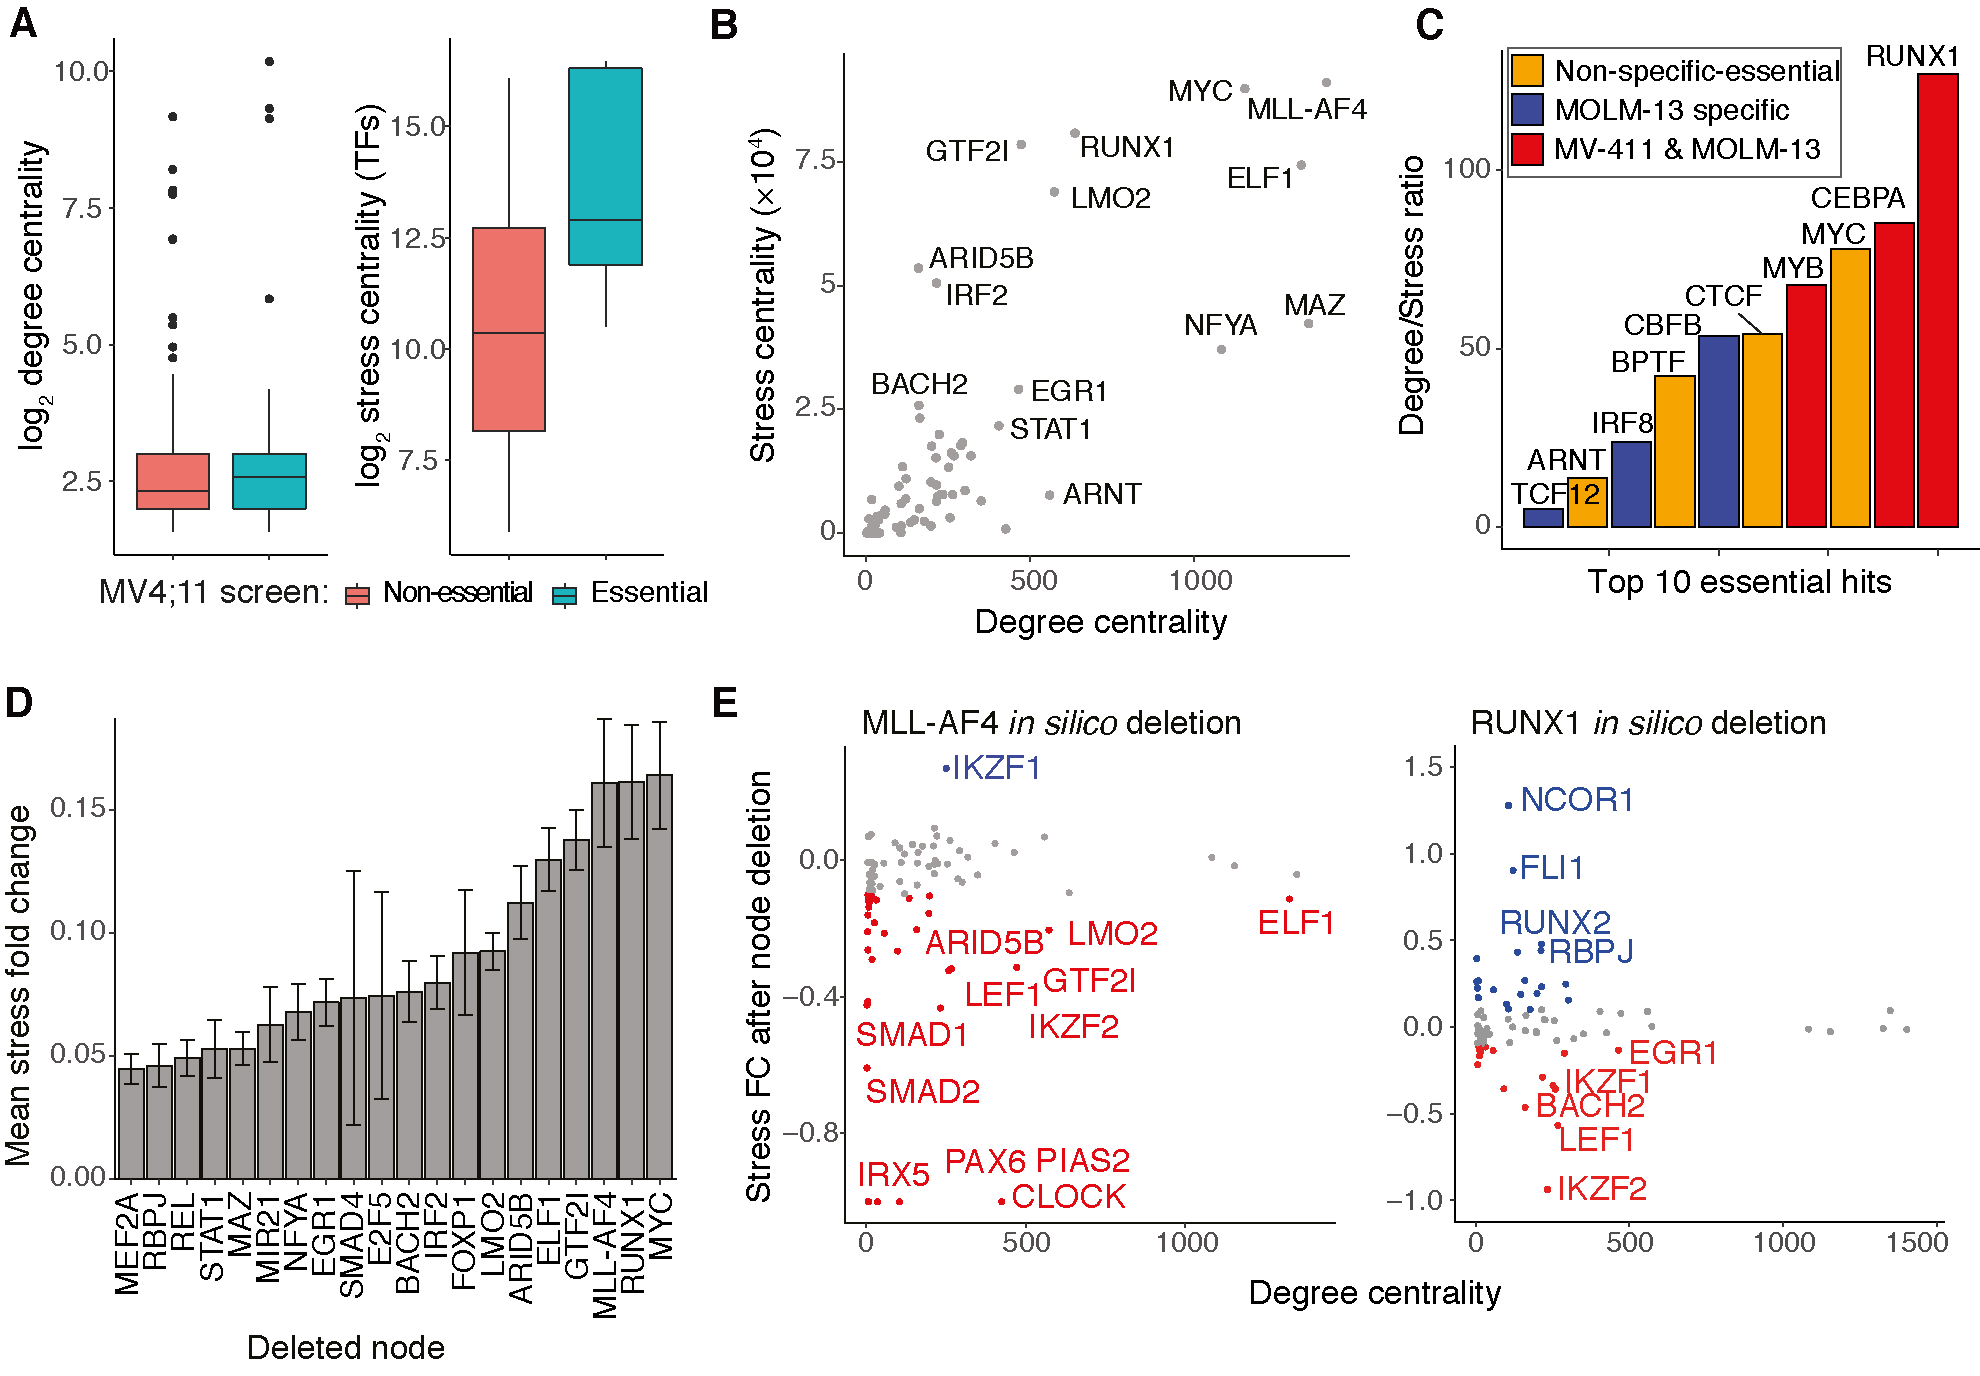
\includegraphics[width=\textwidth,height=\textheight,keepaspectratio]{figures/chapter4/ch4_centrality.png}
    %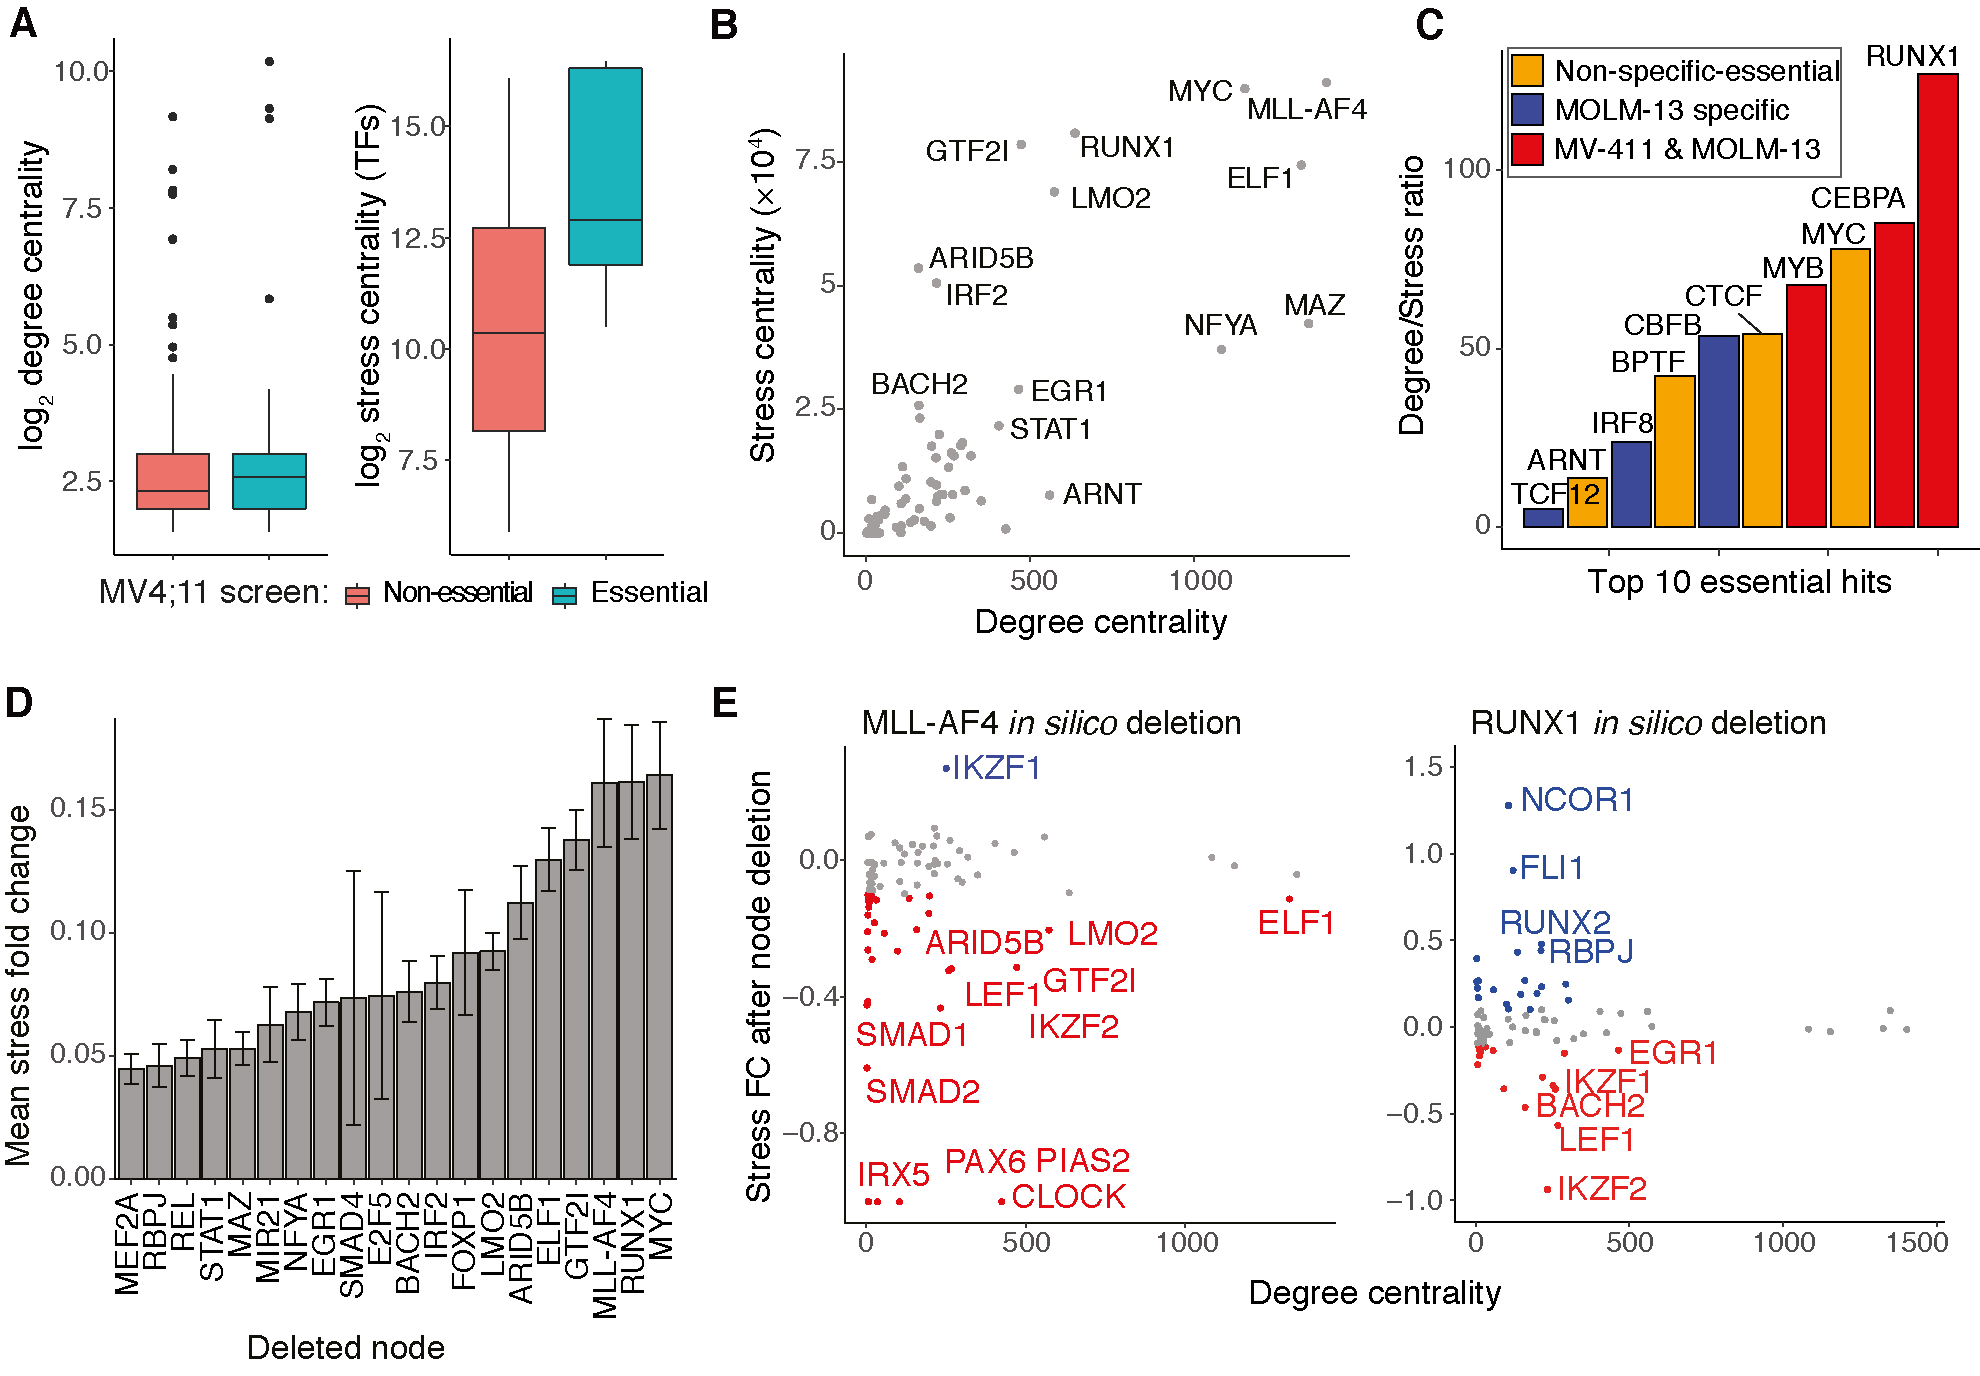
\includegraphics{figures/chapter4/ch4_centrality.png}
    \caption[{Centrality analysis of MLL-AF4 GRN.}]
    {\textbf{Centrality analysis of MLL-AF4 GRN.} 
    \textbf{(A)} Log\textsubscript{2} degree and stress centrality of the MLL-AF4 GRN nodes plotted by essentiality result from \cite{tzelepis_crispr_2016}. 
    \textbf{(B)} Relationship between degree and stress centrality of MLL-AF4 GRN nodes. 
    \textbf{(C)} Rank order plot of top ten ratios between stress and degree centrality for \cite{tzelepis_crispr_2016} for essential GRN hubs. 
    \textbf{(D)} Top 20 in silico deleted nodes by average stress FC (see methods). 
    \textbf{(E)} Stress FC after in silico deletion of RUNX1 or MLL-AF4, plotted against degree centrality. Blue and red indicate positive (FC > 0.1) and negative (FC < -0.1) stress FC, respectively. 
    \textit{Adapted from \cite{harman_kmt2a-aff1_2021}.}
    }
    \label{fig:ch4_centrality}
\end{figure}

While the GRN may be less likely to compensate for loss of high stress hubs, there are TFs with redundant regulatory logic that may act in place of these genes. To investigate this, I established an approach where each GRN node was deleted in silico, and stress centrality recalculated. Stress values before and after in silico deletion were compared as stress fold change (stress FC), and summarised for every node (Fig. \ref{fig:ch4_centrality}D). RUNX1 and MYC in silico deletion showed the greatest stress redistribution, above MLL-AF4, while the non-essential factors MAZ and NFYA show less stress FC redistribution (Fig. \ref{fig:ch4_centrality}D). Looking in detail, MLL-AF4 deletion results in negative stress FC while RUNX1 shows positive and negative stress FC. RUNX1 in silico deletion shows increased NCOR1, FLI1, and RUNX2 stress, while factors such as IKZF1 and IKZF2 are reduced (Fig. \ref{fig:ch4_centrality}E). RUNX2 is expected as it shares the RUNT domain with RUNX1. FLI1 binding in particular has a strong relationship with RUNX1, as the expression of \textit{RUNX1} is reported to shift FLI1 binding preference from ETS/GATA to RUNX1/ETS motifs \citep{gilmour_co-operation_2018, lichtinger_runx1_2012}. RBPJ is a transcriptional repressor on its own, but forms a transactivating complex with NOTCH intracellular domain (NICD) \citep{kojika_notch_2001}. RUNX1 is enriched at RBPJ-NICD binding sites, and both factors have been found to coregulate the +1.27Mb \textit{MYC} enhancer and \textit{IL7R} enhancers \citep{choi_runx1_2017, wang_notch1-rbpj_2014}. Genes that decrease in stress are difficult to interpret, but I propose this reflects a breakdown in particular pathways. For example, if a subset of node pairs must communicate through a RUNX1:IKZF1 axis then loss of RUNX1 will break down the path of communication via IKZF1. This analysis serves to rank the most important nodes in the GRN based on measures of centrality. In particular it highlights RUNX1, MYB, CEBPA and MYC to be highly important TFs, and notes potential redundancy between RUNX1 and specific factors at a subset of targets. 





\subsection{Validating the importance of central regulatory hubs}

%The data thus far builds a case for a core program common across \textit{MLL}r leukaemias. 
To find which TFs are important for leukaemogenesis I integrated publicly available CRISPR essentiality screens. The Cancer Dependency Map (DepMap, Avana 21Q1 dataset, \cite{meyers_computational_2017, doench_optimized_2016}) found \textit{MYC} to be pan-essential, \textit{RUNX1} to be essential in multiple haematopoietic cancer models, and \textit{ELF1} and \textit{MAZ} to be non-essential (Fig. \ref{fig:ch4_essentiality}A). As this is a large and generalised screen, I integrated a more targeted screen from \cite{tzelepis_crispr_2016} which includes two \textit{MLL}r cell lines, MOLM-13 (MLL-AF9 AML) and MV4-11 (MLL-AF4 AML), alongside two non-leukaemic cancer cell lines, HT-29 (colon adenocarcinoma) and HT-1080 (fibrosarcoma). To find genes essential specifically in leukaemia, essential hits were categorised as non-essential, non-specific essential (hit in HT-29 or HT-1080), or essential in one of both \textit{MLL}r leukaemias (hit in MOLM-13 or MV4-11, but not HT-29 or HT-1080) (Fig. \ref{fig:ch4_essentiality}B-C). In line with the DepMap data \textit{MYC} is pan-essential, while \textit{MAZ} and \textit{ELF1} were not essential in any cell line. This suggests \textit{MAZ} and \textit{ELF1}, while highly connected, are not important for survival or proliferation, at least in AML. \textit{RUNX1} was essential in both MOLM-13 and MV4-11 cells, highlighting its importance under the control of both MLL-AF4 and -AF9 fusion proteins. Other central leukaemia-specific hits include \textit{MYB}, \textit{MED13L}, \textit{CEBPA}, and \textit{KAT6A} (Fig. \ref{fig:ch4_essentiality}C). 

\begin{figure}[htbp]
    \centering
    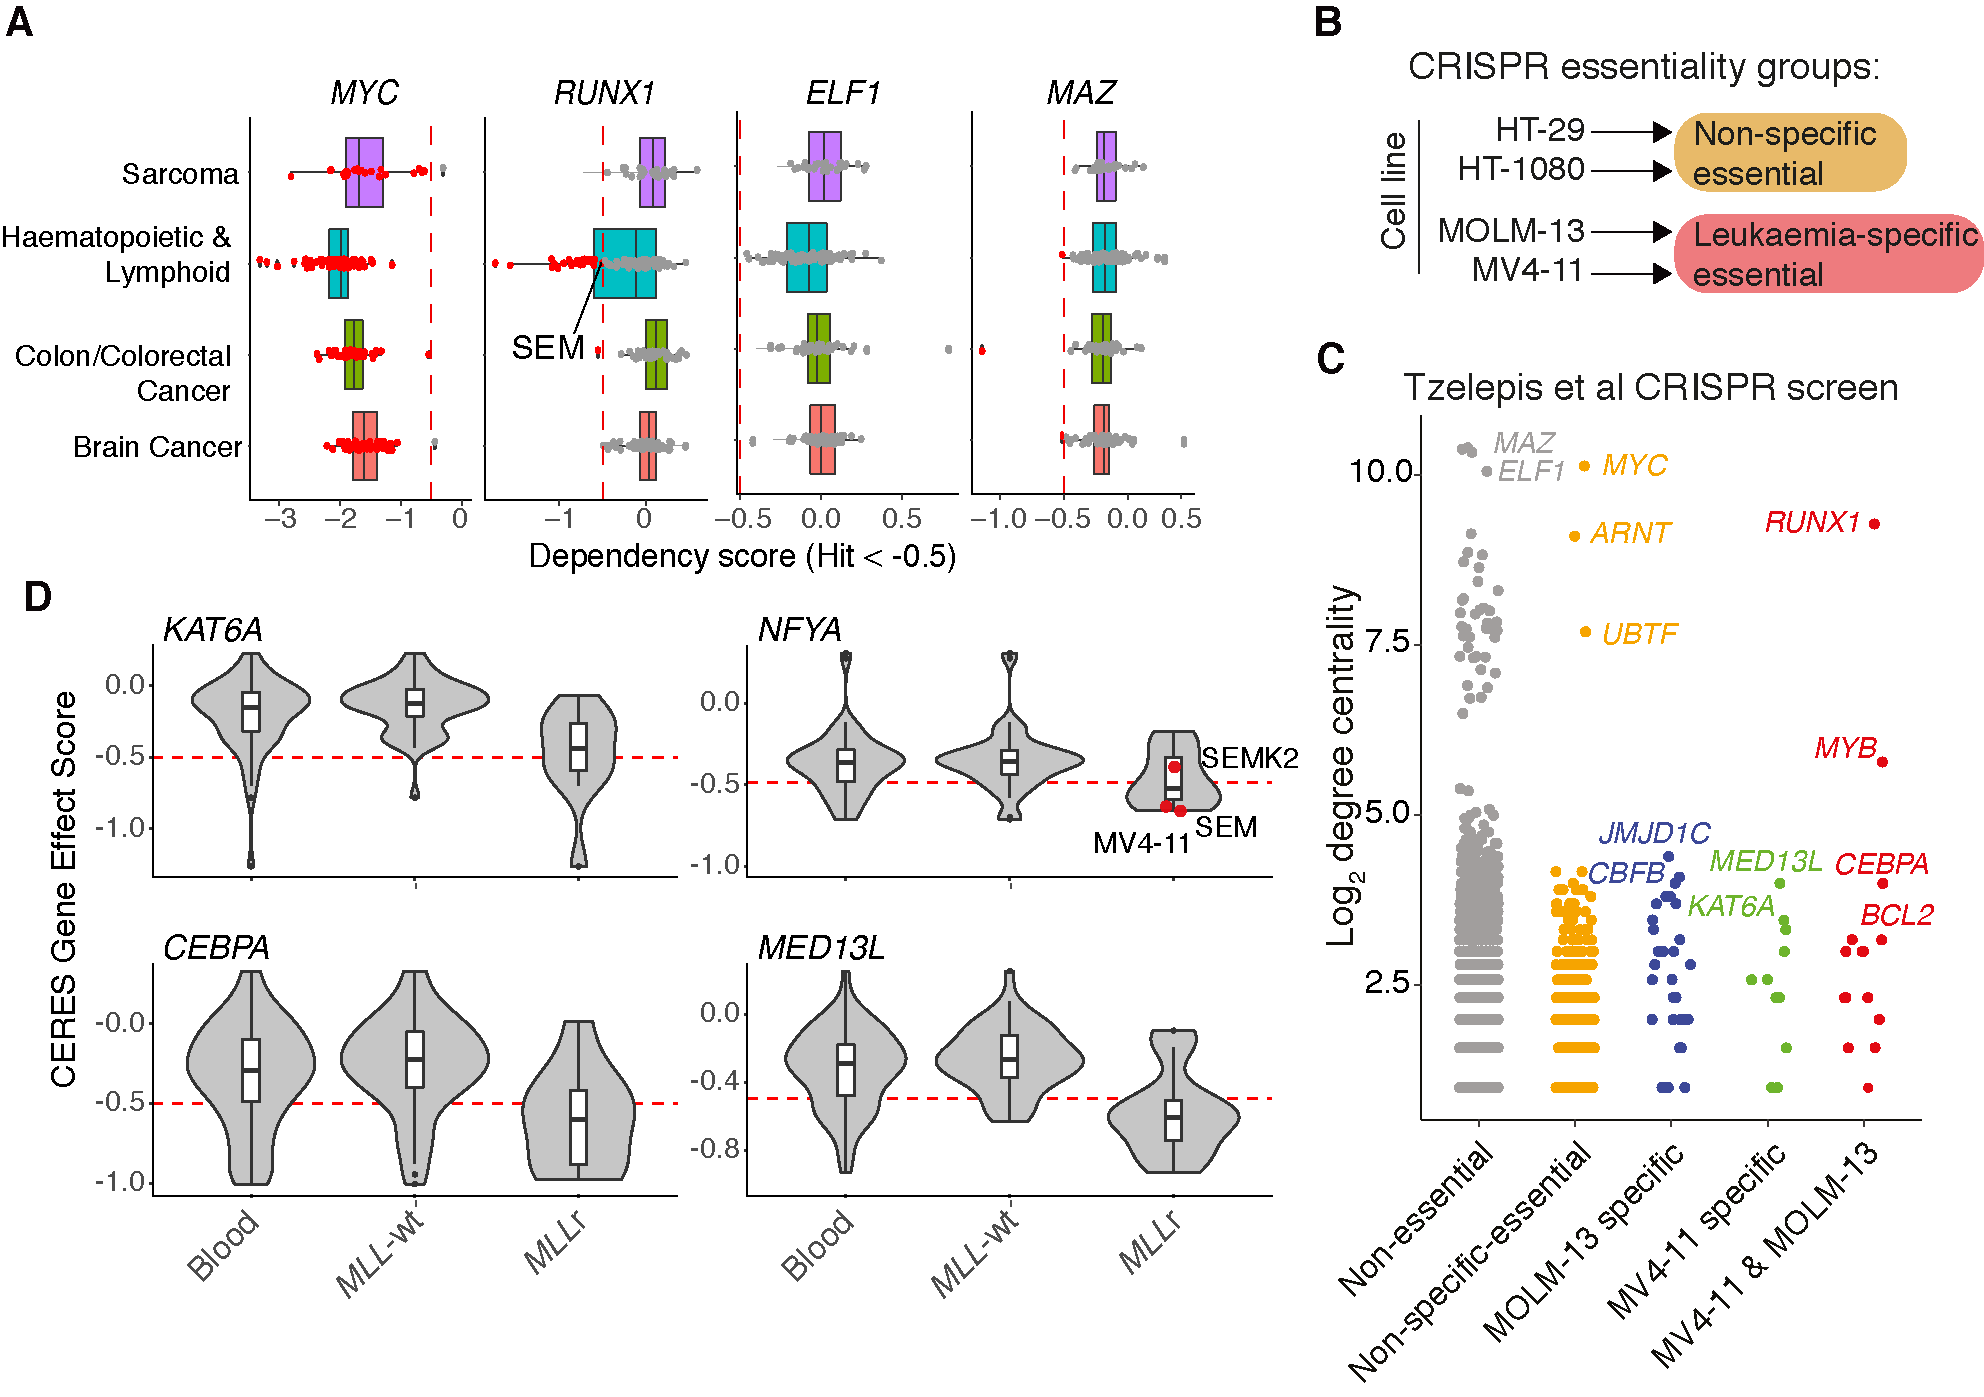
\includegraphics[width=\textwidth,height=\textheight,keepaspectratio]{figures/chapter4/ch4_essentiality.png}
    %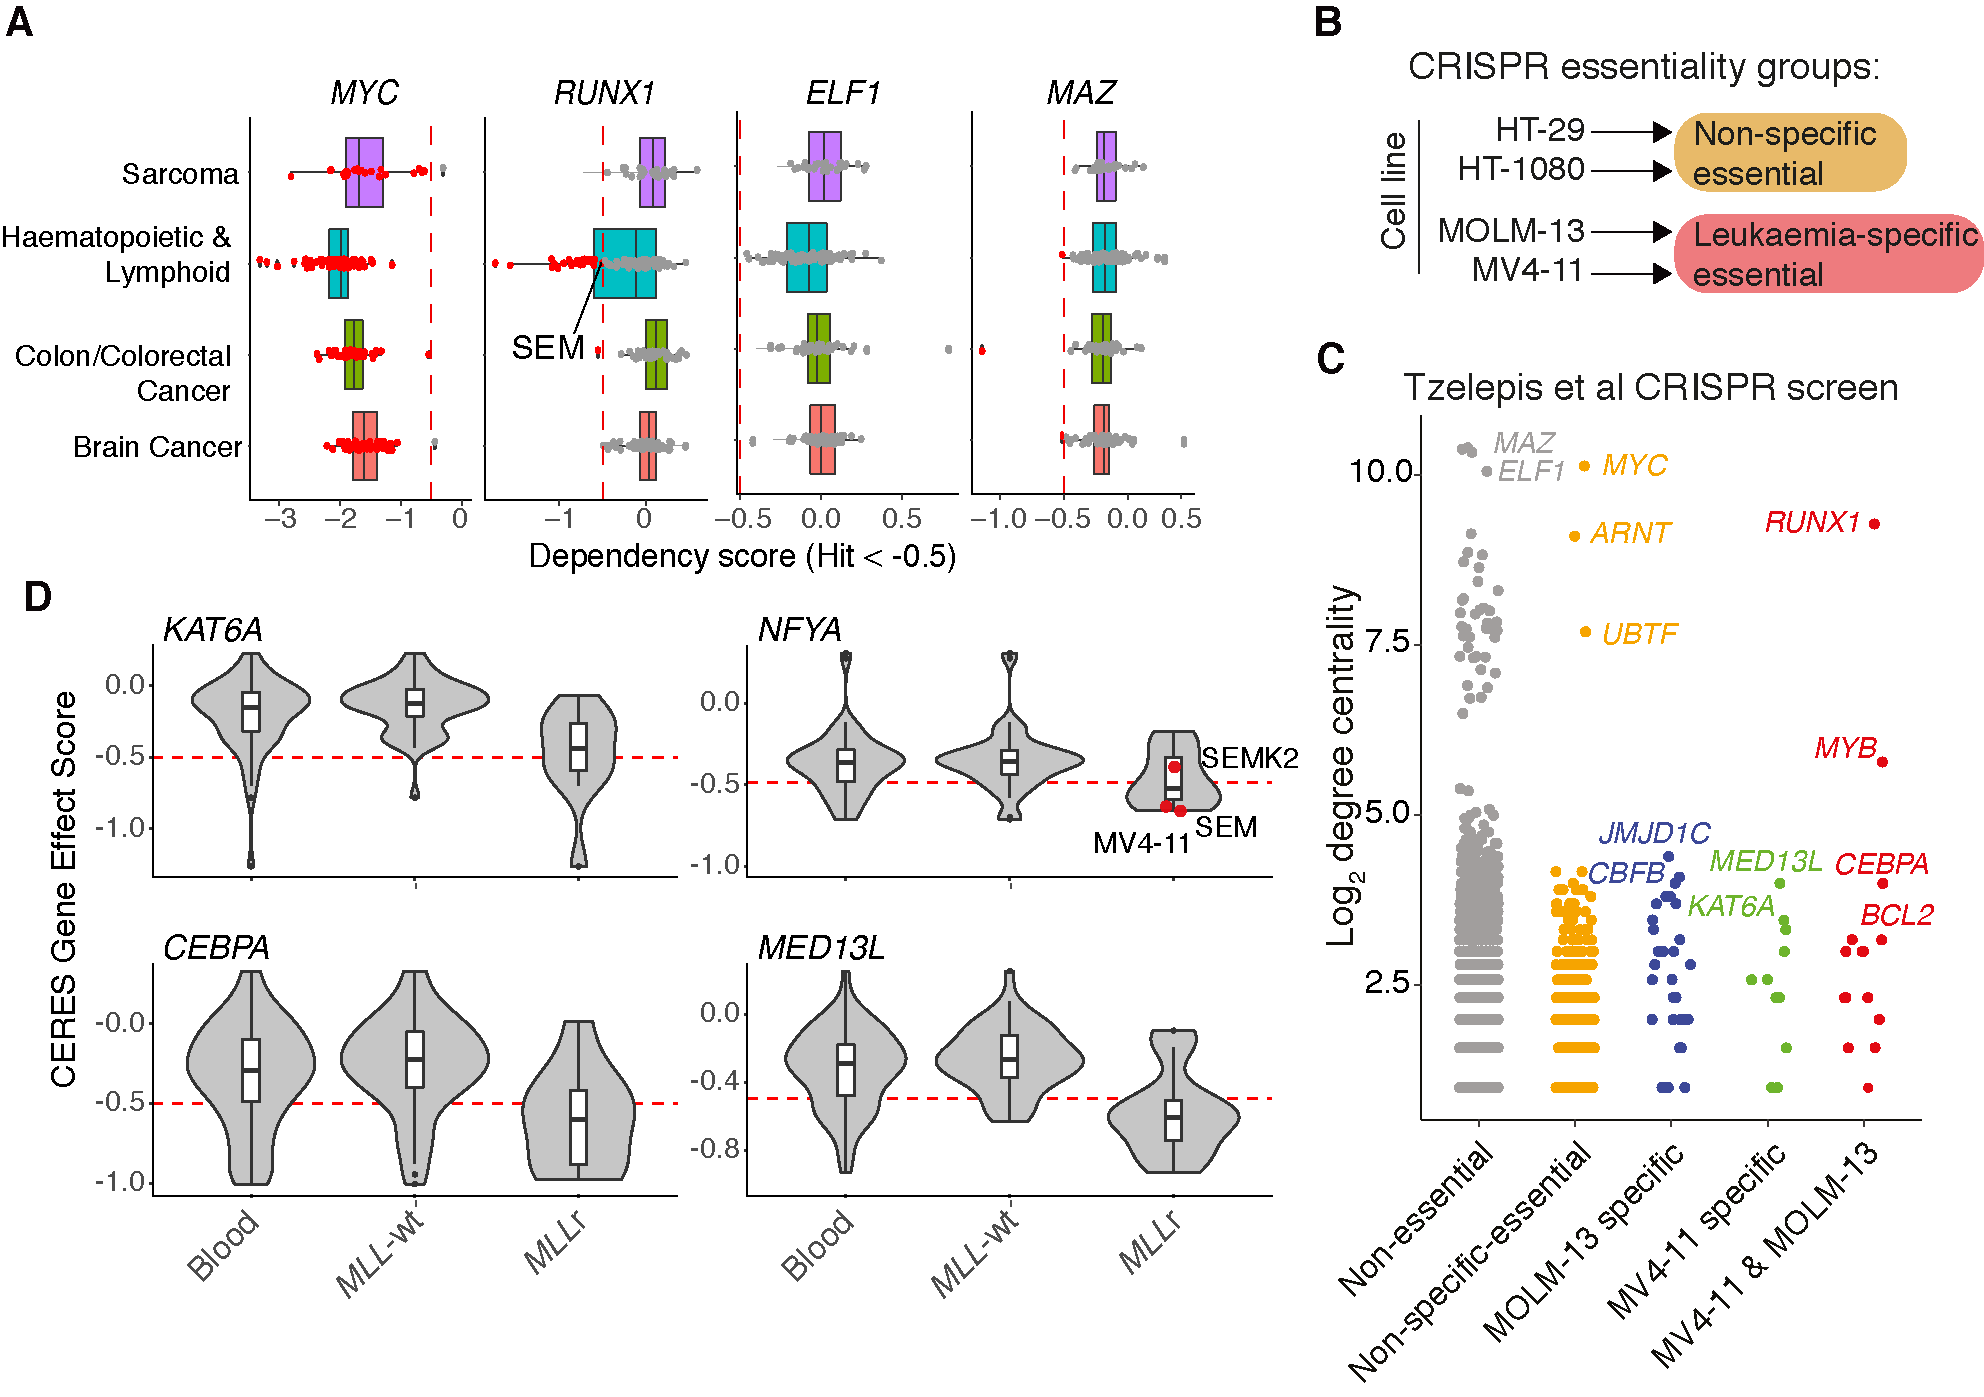
\includegraphics{figures/chapter4/ch4_essentiality.png}
    \caption[{Essential genes.}]
    {\textbf{CRISPR essentiality screens highlight RUNX1 as a critical central TF in MLL-FP leukaemias.} 
    \textbf{(A)} CRISPR essentiality CERES scores from DepMap (Avana 21Q1, \cite{meyers_computational_2017, doench_optimized_2016}). Genes are considered essential with a score below -0.5. Each datapoint represents a different cell line, with essential hits highlighted red.
    \textbf{(B)} Illustration for how CRISPR essentiality screen hits from \cite{tzelepis_crispr_2016} are categorized. Essential genes in HT-29 or HT-1080 were "non-specific essential". Genes not essential in HT-29 or HT-1080 but essential in MOLM-13 or MV4-11 were specific to leukemia. 
    \textbf{(C)} Stratification of log\textsubscript{2} degree centrality (MLL-AF4 GRN) by CRISPR essentiality groups as outlined in B. 
    \textbf{(D)} CERES scores in haematopoietic cancer cell lines from DepMap, stratified by MLL translocation status. 
    \textit{Analysis in D performed by Tom Wilson, supervised by myself. CRISPR scores sourced from DepMap and \cite{tzelepis_crispr_2016}. Adapted from \cite{harman_kmt2a-aff1_2021}.} 
    }
    \label{fig:ch4_essentiality}
\end{figure}

The MV4-11 and MOLM-13 essential gene \textit{CEBPA}, along with the MV4-11 specific hits \textit{MED13L} and \textit{KAT6A}, show greater essentiality for \textit{MLL}r samples over non-\textit{MLL}r blood cancers (Fig. \ref{fig:ch4_essentiality}D). NF-YA is a central (but not core to all MLL-FPs) node in the GRN and is not significantly essential in the \cite{tzelepis_crispr_2016} screen, however the DepMap screens shows higher essentiality in \textit{MLL}r samples with \textit{MLL-AF4} rearrangements showing the highest scores. This indicates that not only are these genes essential for MLL\textit{r} AML, but show greater essentiality for \textit{MLL}r leukaemias than other haematopoietic malignancies, possibly in part as a core-program targeted by MLL-FPs. 